\documentclass[tikz, dvisvgm, border=5mm]{standalone}
\usetikzlibrary{calc, angles, quotes}

\begin{document}
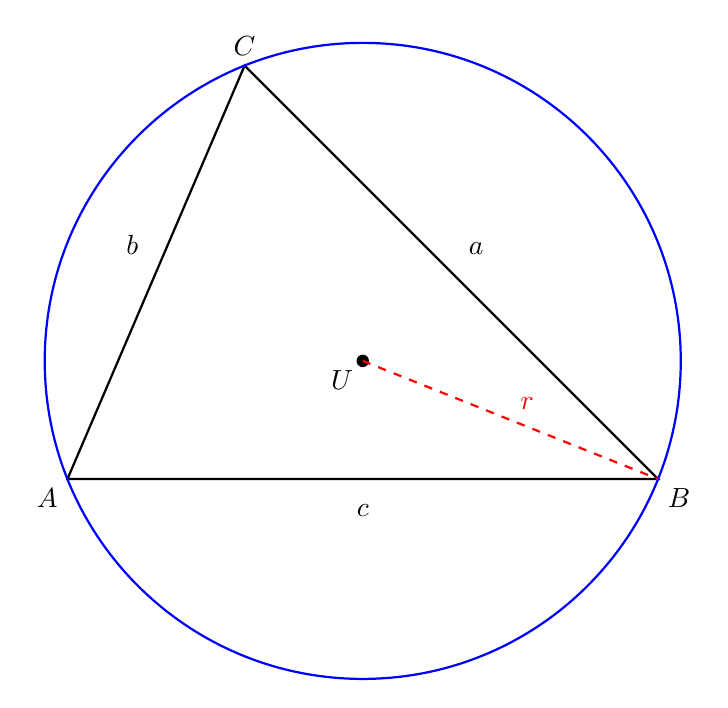
\begin{tikzpicture}[scale=1.5]

    % 1. Definition der Eckpunkte (Allgemeines/schiefwinkliges Dreieck)
    \coordinate (A) at (0,0);
    \coordinate (B) at (5,0);
    \coordinate (C) at (1.5,3.5);

    % Berechneter Umkreismittelpunkt (U) für diese exakten Koordinaten
    \coordinate (U) at (2.5,1);

    % 2. Zeichnen des Dreiecks
    \draw[thick] (A) -- (B) -- (C) -- cycle;

    % 3. Ergänzung: Umkreis und Umkreisradius
    % Umkreis (Radius ist der Abstand von U zu den Eckpunkten, ca. 2.6926)
    \draw[blue, thick] (U) circle (2.6926);
    
    % Umkreismittelpunkt markieren
    \fill[black] (U) circle (1.5pt) node[below left] {$U$};
    
    % Umkreisradius (beispielhaft vom Mittelpunkt zum Punkt B gezeichnet)
    \draw[red, thick, dashed] (U) -- (B) node[midway, above right] {$r$};

    % 4. Beschriftung der Ecken und Seiten
    % Ecken
    \node[below left] at (A) {$A$};
    \node[below right] at (B) {$B$};
    \node[above] at (C) {$C$};
    
    % Seiten (mittig platziert mit leichtem Versatz nach außen)
    \path (A) -- (B) node[midway, below=2mm] {$c$};
    \path (B) -- (C) node[midway, above right=1mm] {$a$};
    \path (C) -- (A) node[midway, above left=1mm] {$b$};

\end{tikzpicture}
\end{document}